% ------------------------------------------------------------------------
% ------------------------------------------------------------------------
% abnTeX2: Modelo de Relatório Técnico/Acadêmico em conformidade com 
% ABNT NBR 10719:2011 Informação e documentação - Relatório técnico e/ou
% científico - Apresentação
% ------------------------------------------------------------------------ 
% ------------------------------------------------------------------------

\documentclass[
	% -- opções da classe memoir --
	12pt,				% tamanho da fonte
	openright,			% capítulos começam em pág ímpar (insere página vazia caso preciso)
	%twoside,			% para impressão em verso e anverso. Oposto a oneside
	oneside,
	a4paper,			% tamanho do papel. 
	% -- opções da classe abntex2 --
	%chapter=TITLE,		% títulos de capítulos convertidos em letras maiúsculas
	%section=TITLE,		% títulos de seções convertidos em letras maiúsculas
	%subsection=TITLE,	% títulos de subseções convertidos em letras maiúsculas
	%subsubsection=TITLE,% títulos de subsubseções convertidos em letras maiúsculas
	% -- opções do pacote babel --
	english,			% idioma adicional para hifenização
	french,				% idioma adicional para hifenização
	spanish,			% idioma adicional para hifenização
	brazil,				% o último idioma é o principal do documento
	]{abntex2}

% ---
% PACOTES
% ---

% ---
% Pacotes fundamentais 
% ---
\usepackage{lmodern}			% Usa a fonte Latin Modern
\usepackage[T1]{fontenc}		% Selecao de codigos de fonte.
\usepackage[utf8]{inputenc}		% Codificacao do documento (conversão automática dos acentos)
\usepackage{indentfirst}		% Indenta o primeiro parágrafo de cada seção.
\usepackage{color}				% Controle das cores
\usepackage{graphicx}			% Inclusão de gráficos
\usepackage{microtype} 			% para melhorias de justificação
% ---

% ---
% Pacotes adicionais, usados no anexo do modelo de folha de identificação
% ---
\usepackage{multicol}
\usepackage{multirow}
% ---
	
% ---
% Pacotes adicionais, usados apenas no âmbito do Modelo Canônico do abnteX2
% ---
\usepackage{lipsum}				% para geração de dummy text
% ---

% ---
% Pacotes de citações
% ---
\usepackage[brazilian,hyperpageref]{backref}	 % Paginas com as citações na bibl
\usepackage[alf]{abntex2cite}	% Citações padrão ABNT

% --- 
% CONFIGURAÇÕES DE PACOTES
% --- 

% ---
% Configurações do pacote backref
% Usado sem a opção hyperpageref de backref
\renewcommand{\backrefpagesname}{Citado na(s) página(s):~}
% Texto padrão antes do número das páginas
\renewcommand{\backref}{}
% Define os textos da citação
\renewcommand*{\backrefalt}[4]{
	\ifcase #1 %
		Nenhuma citação no texto.%
	\or
		Citado na página #2.%
	\else
		Citado #1 vezes nas páginas #2.%
	\fi}%
% ---

% ---
% Informações de dados para CAPA e FOLHA DE ROSTO
% ---
\titulo{Sistema solar minimalista em LaTeX \\utilizando pacote TikZ }
\autor{Paulo Belfi Dias da Silva}
\local{São Paulo -- Brasil}
\data{2017}
\instituicao{%
  Centro Universitário Senac
 \par
  Bacharelado em Ciência da Computação}
\tipotrabalho{Relatório técnico}
% O preambulo deve conter o tipo do trabalho, o objetivo, 
% o nome da instituição e a área de concentração 
\preambulo{Relatório técnico, em conformidade com as normas ABNT, apresentado como requisito para aprovação na disciplina Projeto Integrador I.}
% ---

% ---
% Configurações de aparência do PDF final

% alterando o aspecto da cor azul
\definecolor{blue}{RGB}{41,5,195}

% informações do PDF
\makeatletter
\hypersetup{
     	%pagebackref=true,
		pdftitle={\@title}, 
		pdfauthor={\@author},
    	pdfsubject={\imprimirpreambulo},
	    pdfcreator={LaTeX with abnTeX2},
		pdfkeywords={abnt}{latex}{abntex}{abntex2}{relatório técnico}, 
		colorlinks=true,       		% false: boxed links; true: colored links
    	linkcolor=blue,          	% color of internal links
    	citecolor=blue,        		% color of links to bibliography
    	filecolor=magenta,      		% color of file links
		urlcolor=blue,
		bookmarksdepth=4
}
\makeatother
% --- 

% --- 
% Espaçamentos entre linhas e parágrafos 
% --- 

% O tamanho do parágrafo é dado por:
\setlength{\parindent}{1.3cm}

% Controle do espaçamento entre um parágrafo e outro:
\setlength{\parskip}{0.2cm}  % tente também \onelineskip

% ---
% compila o indice
% ---
\makeindex
% ---

% ----
% Início do documento
% ----
\begin{document}

% Retira espaço extra obsoleto entre as frases.
\frenchspacing 

% ----------------------------------------------------------
% ELEMENTOS PRÉ-TEXTUAIS
% ----------------------------------------------------------
% \pretextual

% ---
% Capa
% ---
\imprimircapa
% ---

% ---
% Folha de rosto
% (o * indica que haverá a ficha bibliográfica)
% ---
\imprimirfolhaderosto%*
% ---

% ---
% Anverso da folha de rosto:
% ---

% ---
% RESUMO
% ---

% resumo na língua vernácula (obrigatório)
\setlength{\absparsep}{18pt} % ajusta o espaçamento dos parágrafos do resumo
\begin{resumo}
Gerar um código que reproduza o movimento de translação dos planetas, por mais que desconsidere algumas circunstancias, podem acabar gerando alguns problemas por mais simples que pareça.
Este relatório tem como objetivo demonstrar como foi reproduzir parte do movimento de translação dos planetas. E quais as dificuldades encontradas para gerar o código em \LaTeX, e transformá-lo em um PDF.

 \noindent
 \textbf{Palavras-chaves}: latex. tikz. Sistema Solar. Minimalismo.
\end{resumo}
% ---

% ---
% inserir o sumario
% ---
\pdfbookmark[0]{\contentsname}{toc}
\tableofcontents*
\cleardoublepage
% ---

% ----------------------------------------------------------
% ELEMENTOS TEXTUAIS
% ----------------------------------------------------------
\textual

% ----------------------------------------------------------
% Introdução
% ----------------------------------------------------------
\chapter[Introdução]{Introdução}
%\addcontentsline{toc}{chapter}{Introdução}
% ----------------------------------------------------------

Este documento demonstra como foi criada a animação do sistema solar minimalista, utilizando o pacote Tikz dentro da linguagem LaTex. Com seu código sendo gerado através de um programa em linguagem C. A motivação de realizar este trabalho foi devido a gostar do estudo de astronomia, e querer reproduzir esta ideia para um código que conseguisse demonstrar um pouco do universo.

Para gerar o código em Tikz LaTeX, foi necessário um programa em C, para automatizar o processo de gerar o cálculo da posição de cada planeta, utilizando conceitos de ângulos e círculo trigonométrico. E para gerar os slides da animação foram utilizados, códigos básicos, como \textit{fill}, \textit{definecolor}, \textit{frame}.




% ----------------------------------------------------------
% Capitulo 2
% ----------------------------------------------------------
\chapter[Materiais e Métodos]{Materiais e Métodos}
% ----------------------------------------------------------

Para gerar a animação foram utilizados diversas ferramentas. Iniciando pela definição de como seria o modelo a ser utilizado, usando o site overleaf.com, para definir as dimensões e cores que seriam utilizados pelos, planetas. \\
\indent Após essa definição foi necessário o uso de um programa em C que iria gerar o código TikZ, a ser reproduzido. \\
\indent E finalmente para compilar o código gerado, foi utilizado o compilador pdflatex, pois nenhum dos editores de código LaTeX testados suportavam o arquivo.

\section{Motivações ao uso do material}

 As ferramentas utilizadas em sua maioria foram escolhidas devido a familiaridade do autor.
 \\ \indent A escolha do site overleaf.com, foi devido a facilidade de uso do mesmo, por mais que não tenha o melhor desempenho em questão de tempo de compilação o site atende bem as expectativas de usuários que não tenham tanta familiaridade com o LaTeX.
 \\ \indent Para escrever o código em C foi utilizado o software "Sublime Text 3", devido a sua facilidade de uso e conter diversos facilitadores para a escrita de código fonte em C.
 \\ \indent Para compilar o código LaTeX foi utilizado o compilador pdflatex em uma plataforma Linux, pois foi o único testado que conseguia compilar o código gerado.


% ----------------------------------------------------------
% Capitulo 3
% ----------------------------------------------------------
\chapter[Desenvolvimento]{Desenvolvimento}
% ----------------------------------------------------------

O desenvolvimento foi inicialmente definir as cores, proporções e medidas que seriam utilizadas para gerar o código e posteriormente a definição da animação em latex. 

\section{Tipo de documento e pacotes usados}
	Como irá ser criada uma animação faz se necessário criar um documento que suporte animações, o escolhido foi o beamer, pois o seu uso é simples, e atendeu as necessidades do trabalho.
	\\ \indent Para definir as cores que serão utilizadas nos planetas foi utilizado o pacote xcolor, pois assim consegue-se converter as cores em RGB, que serão extraídas da imagem de referencia para cores aceitadas em LaTeX.
	\\ \indent Para a realização do desenho foi utilizado o pacote TikZ pois era uma das obrigatoriedades do trabalho, e é um pacote de fácil utilização.


\section{Criação do modelo a ser usado}
	Para criar o modelo foi utilizado o site overleaf.com, aonde foi definido todo o primeiro slide da animação, ele será utilizado como base de todo o trabalho.
	\\ \indent  Utilizando dados reais dos tamanhos dos planetas, foi gerado uma imagem de teste aonde os planetas seguiam a mesma proporção do tamanho real. Porém quando a imagem era gerada, ficava imperceptível a existência de alguns planetas na imagem. Então a saída para este problema foi utilizar de licença poética e dar tamanhos não proporcionais aos planetas.\\
	\begin{figure}
		\centering
		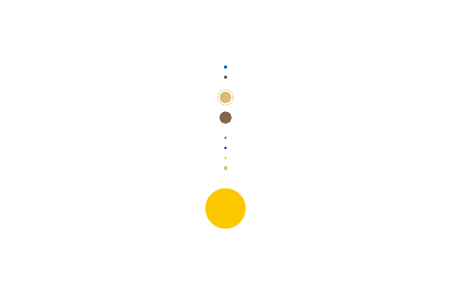
\includegraphics[width=0.5\linewidth]{../../../../../Desktop/Relatorio/ImagemBase}
		\caption{Imagem gerada como base}
		\label{fig:imagembase}
	\end{figure}
	\\ \indent Definido o desenho a ser realizado pelo TikZ, foi preciso apenas definir o uso do primeiro slide e tempo de transição de cada slide. Cada slide contem a posição do planeta em determinado dia, ou seja cada slide é equivalente a um dia na Terra. Como alguns planetas demoram mais do que outros para completarem o seu movimento de translação, sendo o mais demorado do sistema solar Netuno, que demora cerca de 160 anos da Terra, para completar o movimento, foi necessário realizar uma aceleração, na transição dos slides. Inicialmente foi testado, o tempo de transição de cada slide em 24 slides por segundo, porém o tempo de duração total acaba sendo muito grande, cerca de 41 minutos, para completar o movimento de Netuno. Então foi alterado o tempo de duração para 60 slides por segundo, que totalizava cerca de 13 minutos, ainda bastante tempo, porém com maior fluidez no movimento.
		
\section{Criação do algoritmo que irá gerar o código LaTeX}
	Após definido o modelo base de uso do sistema solar, o tempo de transição de cada slide, o próximo passo foi gerar o código que irá gerar o código LaTeX a ser gerado. Para isso foi utilizado o software "Sublime Text 3", um software de edição de texto, e o mesmo possui diversas ferramentas que auxiliam no momento de escrever o código em linguagem C. E o compilador de linguagem C, GCC em sua versão 6.3.0, em uma plataforma Windows.
	\\ \indent Para gerar a simulação do movimento de translação dos planetas, existem dois cenários possíveis, o cenário aonde será simulado o movimento da forma mais fidedigna possível, e o cenário que irá simular um movimento que remeta ao movimento de translação. O primeiro cenário implica em conseguir traduzir para o algoritmo, diversos fatores, como massa dos planetas, movimentos elípticos, aceleração devido a distância entre corpos celestes, e outros diversos fatores.
	Já o segundo cenário, contém somente a ideia do movimento de translação simplificado, do qual funciona de forma semelhante a um circulo trigonométrico.
	\\ \indent A posição de cada planeta, será definido pela sua posição (X,Y), sendo X o seno do ângulo relativo ao dia multiplicado pela sua distancia do centro do Sol. Isso significa o total de slides, desde o inicio da animação, dividido pelo tempo de duração do ano do planeta e multiplicado pela distância do planeta ao Sol. E Y a mesma formula que X, porem alterando seno por cosseno.
	\\ \indent Definido o método que deverá ser reproduzido, podemos partir então para a codificação do movimento, o código TikZ LaTeX, foi separado em duas partes, a que não possui repetição, área do código onde será definido os padrões que serão utilizados na animação, como por exemplo classe do documento, cores dos planetas, definições dos pacotes e etc. E a parte que será repetida, que é composta pela definição dos frames e das figuras a serem geradas.\\
	\begin{figure}[h]
		\centering
		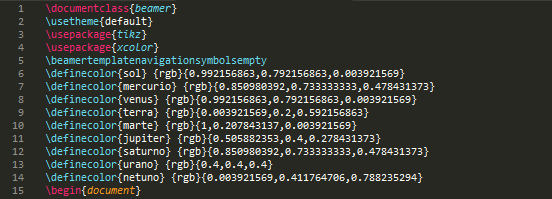
\includegraphics[width=0.5\linewidth]{../../../../../Desktop/Relatorio/Inicio_codigo}
		\caption{Parte fixa do código LaTeX}
		\label{fig:Inicio_codigo}
	\end{figure}

	\begin{figure}[h]
		\centering
		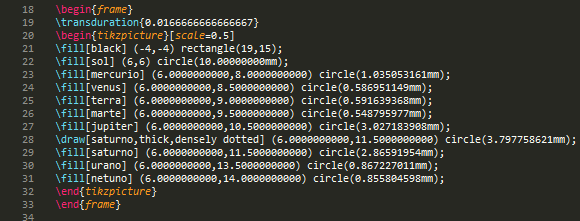
\includegraphics[width=0.5\linewidth]{../../../../../Desktop/Relatorio/Repeticao_codig}
		\caption{Parte de repetição do código LaTeX}
		\label{fig:Repeticao_codigo}
	\end{figure}
	\indent Já dentro do código em linguagem C, serão utilizados, os pacotes "stdio.h", "stdlib.h", "math.h" e também será utilizado um arquivo ".tex"  para a saída do código gerado, pois irá facilitar o processo para a compilação do código LaTeX. Inicialmente iremos inserir dentro deste arquivo ".tex", a parte fixa do código. Como visto na figura 4 logo acima.
	\begin{figure}[h]
		\centering
		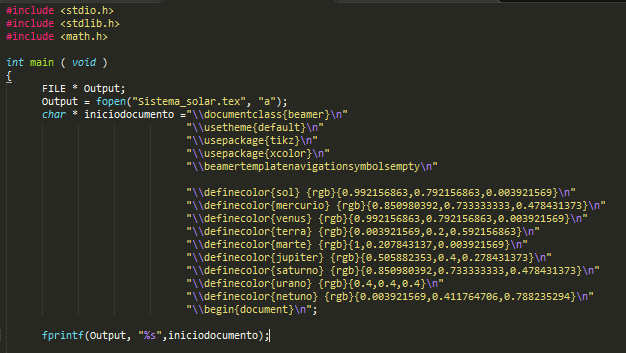
\includegraphics[width=0.5\linewidth]{../../../../../Desktop/Relatorio/screenshot001}
		\caption{Inserção da parte fixa do código}
		\label{fig:screenshot001}
	\end{figure}
	\\ \indent Para a geração dos slides será necessário o algorítimo que gera a posição relativa dos planetas e um loop que irá controlar o angulo relativo de cada planeta. Sendo assim o código em C ficará da seguinte forma. 
	\begin{figure}[h]
		\centering
		\includegraphics[width=0.5\linewidth]{../../../../../Desktop/Relatorio/Repeticao_codigoc}
		\caption{Inserção da parte variável do código}
		\label{fig:Repeticao_codigoc}
	\end{figure}
	 \indent Após isso falta somente compilar o código e executá-lo, para isso foi utilizado o compilador GCC ver. 6.3.0 para Windows. Para compilar o arquivo se utiliza o comando GCC no terminal. Já com o terminal dentro da pasta aonde se localiza o arquivo ".c", utiliza-se o comando GCC passando como parâmetro o nome do arquivo ".c" -o nome do arquivo de saída. Como no exemplo abaixo.
	\begin{figure}[h]
		\centering
		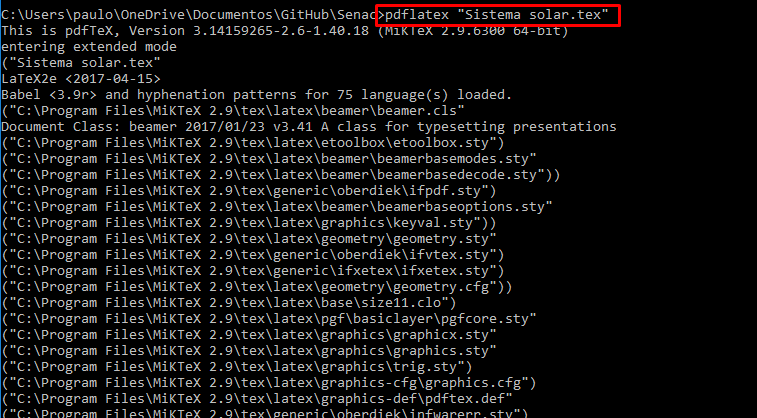
\includegraphics[width=0.7\linewidth]{screenshot002}
		\caption{Compilação do código em C}
		\label{fig:screenshot002}
	\end{figure}
	
	
\section{Compilação do código}
	Como dito anteriormente nenhum dos softwares de edição de código LaTeX testados, foram capazes de abrir o arquivo ".tex" gerado. Então desta forma foi necessário compilar o código diretamente pelo terminal. Inicialmente foi testado no compilador pdflatex, para Windows, porém em determinado momento o compilador não conseguia prosseguir com a compilação do arquivo.
	\\ \indent Então fez se necessário compilar o código LaTeX, no compilador pdflatex para Linux, já neste caso, do tempo de quase 1 hora compilando o arquivo, a compilação foi finalizada com sucesso.
 	\\ \indent Para compilar o arquivo se utiliza o comando pdflatex no terminal. Já com o terminal dentro da pasta aonde se localiza o arquivo ".tex", utiliza-se o comando pdflatex passando como parâmetro o nome do arquivo .tex.\\
\begin{figure}[h]
	\centering
	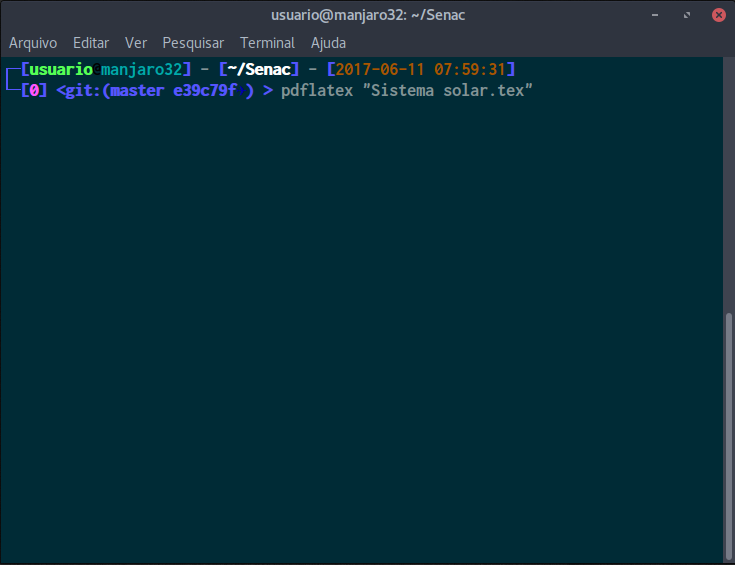
\includegraphics[width=0.5\linewidth]{screenshot003}
	\caption{Compilação do código LaTeX}
	\label{fig:screenshot003}
\end{figure}

	
% ----------------------------------------------------------
% Capitulo 4
% ----------------------------------------------------------
\chapter[Resultado]{Resultado}
% ----------------------------------------------------------
	Como o trabalho desenvolvido é uma animação e não pode ser reproduzida neste relatório irei deixar um link para o download da mesma, e uma imagem demonstrativa do resultado final.
	
	Link de download da animação: bit.ly/2rQkGzQ
	
	\begin{figure}[h]
		\centering
		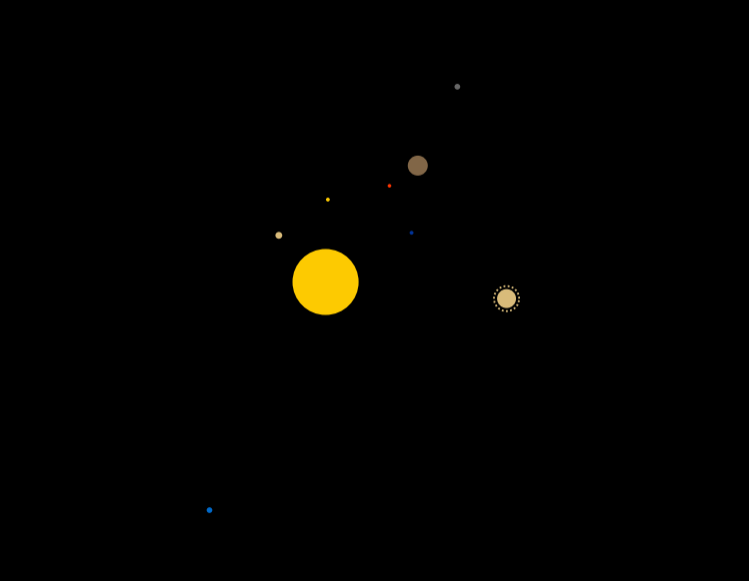
\includegraphics[width=0.5\linewidth]{screenshot004}
		\caption{Demostração do resultado}
		\label{fig:screenshot004}
	\end{figure}
	
	
\section{Detalhes extras}
	O código fonte da animação contém cerca de 962.256 linhas de código, porém o código em linguem C, possui 49 linhas. Para compilar a animação foi necessário cerca de 1 hora. O tempo de duração da animação é de cerca de 14 minutos, possuindo 60140 slides, a 60 slides por segundo.
	\\ \indent foram investidos cerca de 30 horas, para desenvolver o trabalho ao todo, sendo a maior parte buscando como iria ser calculada a posição dos planetas.

% ----------------------------------------------------------
% Capitulo 5
% ----------------------------------------------------------
\chapter[Conclusão]{Conclusão}
% ----------------------------------------------------------
	O TikZ é uma ferramenta ótima, para manipulações de formas geométricas que possamos exemplificar utilizando funções matemáticas, porém em seu uso para reproduzir desenhos, se faz um tanto quanto complexa. Tendo outras ferramentas que são de mais fácil uso.
	\\ \indent Para reprodução de desenhos mais complexos, é necessário um grande estudo da ferramenta e um grande esforço por parte do usuário para se aprimorar na ferramenta, e conseguir executar o desenho.
	\\ \indent O uso da ferramenta é interessante para desenhos que sejam mais simples, que não tenham tantas irregularidades e preferencialmente que possam ser expressadas de formas matemáticas, pois a ferramenta dispõe de uma série de funções para este tipo de imagem.

% ----------------------------------------------------------
% ELEMENTOS PÓS-TEXTUAIS
% ----------------------------------------------------------
\postextual

% ----------------------------------------------------------
% Referências bibliográficas
% ----------------------------------------------------------
\bibliography{abntex2-modelo-references}


\end{document}
